\section{Uvod}
\subsection{Raspberry pi}
Raspberry pi je serija malih \foreign{single-board \footnote{Računalo u potpunosti izgrađeno na jednoj pločici}} 
računala široko korištenih u svrhe eksperimentalnih projekata. \cite{rPiBook}
\paraBreak
Idealan je za tu upotrebu zbog privlačne cijene i odlične portabilnosti te jako male potrošnje struje.
\paraBreak
Za ovaj rad je odabran zbog osim navedenih razloga još i radi ogromnog izbora eksternih modula, specifično službenog kamera modula
koji služi kao baza cijelog projekta.

\begin{figure}[ht]
  \centering
  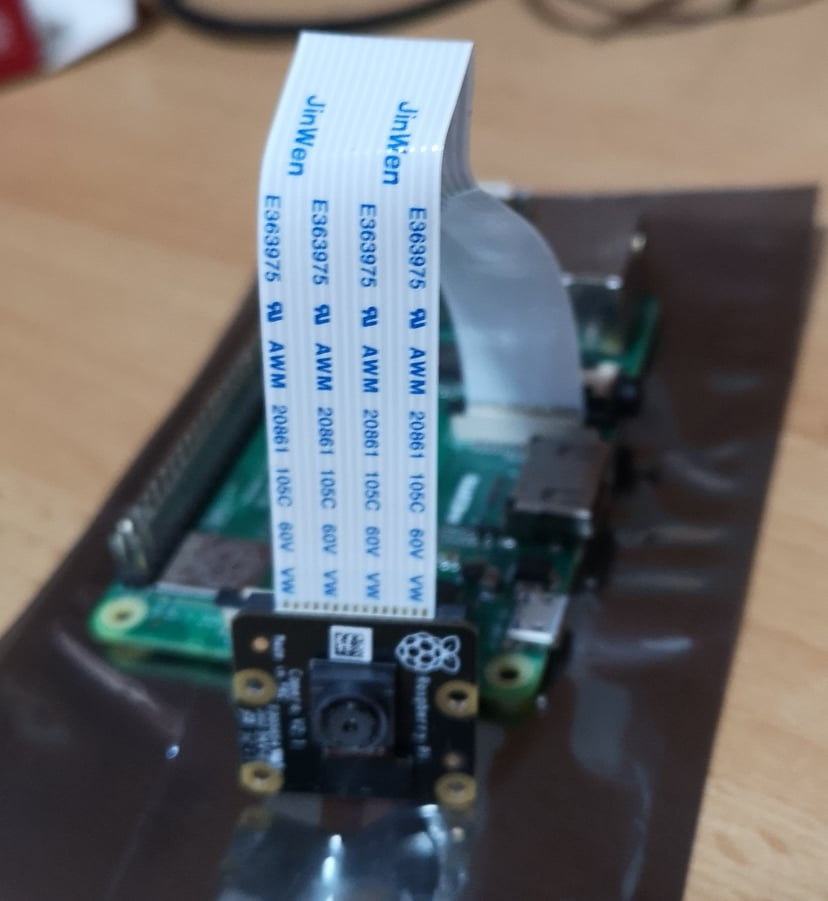
\includegraphics[width=0.6\textwidth]{raspberyy-pi-camera.jpg}
  \caption{Raspberry pi kamera modul}
\end{figure}

\begin{figure}[ht]
  \centering
  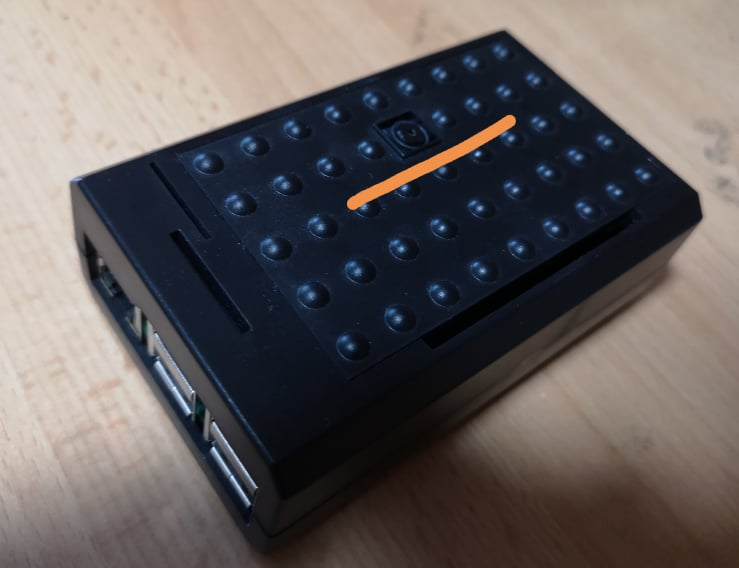
\includegraphics[width=\textwidth]{raspberyy-pie-in-box.jpg}
  \caption{Raspberry pi u kutiji sa otvorom za leću kamere}
\end{figure}

\clearpage
\subsection{FFmpeg} \label{sec:ffmpeg}
FFmpeg je \foreign{open-source} projekt koji se sastoji od mnoštva biblioteka za manipuliranje videom, audiom i ostalom multimedijom.
\cite{ffmpegBook}
\paraBreak
Najveća primjena mu je u transkodiranju, editiranju, skaliranju i raznim efektima videa.
\paraBreak
Najbitnije biblioteke iz FFmpeg-a koje se koriste u ovom radu su \cite{ffmpegDocs}
\begin{itemize}
  \item libavcodec - audio/video kodek biblioteka
  \item libavformat - audio/video kontejner \hyperref[sct:mux]{\foreign{}{mux}} i \hyperref[sct:demux]{\foreign{}{demux}} biblioteka
  \item libavdevice - biblioteka za dohvaćanje i rad dostupnim multimedija uređajima
  \item libswscale - biblioteka za manipulaciju i skaliranje slika videa
\end{itemize}
Koristi se u mnogim popularnim projektima kao što su Google Chrome, VLC Player, YouTube, Blender, HandBrake, Kodi, Plex. \cite{ffmpegBook}

\clearpage
\subsection{Internet stvari} \label{sec:IOT}
Pojam Internet stvari ili \foreign{IoT} se odnosi na milijarde fizičkih uređaja diljem svijeta koji su povezani na Internet
skupljajući ili prosljeđivajući podatke. \cite{IOT}
\paraBreak
Zahvaljujući sve većoj dostupnosti jeftinih malih računala kao što je \foreign{Raspberry pi} moguće je skoro bilo što
od lampe ili pilule pa do aviona pretvoriti u "pametne" uređaje koji su dio interneta stvari.